% 08 --- Simulation Data Analysis
\section{Simulation Data Analysis}

\begin{frame}{Trajectory --- The Movie}
	\begin{columns}[T,onlytextwidth]
		\column{0.5\textwidth}
		\begin{pitemize}
			\item \textbf{Trajectory}: $\{\mathbf{R}(t_0),\mathbf{R}(t_1),\dots\}$ --- DCD/XTC
			\item Size: $N\times 3\times N_{\text{frames}}\times 4$ bytes
			\item \textbf{Analysis} = compress movie \ensuremath{\rightarrow} numbers
		\end{pitemize}
		\column{0.5\textwidth}
		\begin{center}
			\begin{tikzpicture}[scale=1.0]
				% Three snapshot frames showing molecule moving
				\foreach \idx/\dx/\dy in {0/0/0.2,1/2.2/0.0,2/4.4/-0.15} {
						\draw[accentcyan,thick,rounded corners=1mm,fill=darkgray] (\idx*2.0,0) rectangle ++(1.6,1.4);
						\shade[ball color=neonblue] (\idx*2.0+0.5,0.7+\dy) circle (0.12);
						\shade[ball color=neonpink] (\idx*2.0+1.0,0.5+\dy) circle (0.10);
						\shade[ball color=neongreen] (\idx*2.0+0.8,1.0+\dy) circle (0.09);
					}
				% Arrows between frames
				\draw[->,thick,neonyellow] (1.6,0.7) -- (2.0,0.7);
				\draw[->,thick,neonyellow] (3.6,0.7) -- (4.0,0.7);
				\node[color=softgray,font=\footnotesize] at (2.8,-0.3) {$t_0 \to t_1 \to t_2$};
				\node[color=accentcyan,font=\footnotesize] at (0.8,1.7) {frame 0};
				\node[color=accentcyan,font=\footnotesize] at (2.8,1.7) {frame 1};
				\node[color=accentcyan,font=\footnotesize] at (4.8,1.7) {frame 2};
			\end{tikzpicture}
		\end{center}
	\end{columns}
\end{frame}

\subsection{Geometric Measures}
\begin{frame}{RMSD, RMSF, $R_g$}
	\begin{columns}[T,onlytextwidth]
		\column{0.33\textwidth}
		\begin{infobox}[RMSD]
			\footnotesize $\text{RMSD}(t)=\sqrt{\frac1N\sum_i |\mathbf{r}_i(t)-\mathbf{r}_i^{\text{ref}}|^2}$\\\footnotesize drift = motion
		\end{infobox}
		\column{0.33\textwidth}
		\begin{infobox}[RMSF]
			\footnotesize $\text{RMSF}_i=\sqrt{\langle (\mathbf{r}_i-\langle\mathbf{r}_i\rangle)^2\rangle}$\\\footnotesize flexibility per residue
		\end{infobox}
		\column{0.33\textwidth}
		\begin{infobox}[R$_g$]
			\footnotesize $R_g^2=\frac1N\sum_i |\mathbf{r}_i-\mathbf{r}_{\text{COM}}|^2$\\\footnotesize compactness
		\end{infobox}
	\end{columns}
\end{frame}

\begin{frame}{H-Bonds, Distances, Angles}
	\begin{columns}[T,onlytextwidth]
		\column{0.5\textwidth}
		\begin{pitemize}
			\item \textbf{H-bond}: $d_{\text{O}\cdots\text{H}}<3.5$Å, $\angle>150^\circ$
			\item Distances/angles \ensuremath{\rightarrow} \textbf{order parameters}
			\item \textbf{Define} before measuring
		\end{pitemize}
		\column{0.5\textwidth}
		\begin{tikzpicture}[scale=1.0]
			\shade[ball color=neonblue] (0,0) circle (0.32cm) node[color=white]{O};
			\shade[ball color=neonyellow] (1,0.6) circle (0.22cm) node[color=bgblack]{H};
			\draw[dashed,neonpink,thick] (0,0) -- (1,0.6) node[midway,above,sloped]{H-bond};
			\draw[accentcyan,thick] (1,0.6) -- (2,0.2);
			\draw[neonyellow] (1,0.6) -- (1.5,0.3) arc (30:-10:0.4cm);
			\node[color=neonyellow] at (1.6,0.2) {$\theta$};
		\end{tikzpicture}
	\end{columns}
\end{frame}

\subsection{RDF \& Clustering}
\begin{frame}{Radial Distribution Function}
	\begin{equation*}
		g(r)=\frac{\langle \rho(r)\rangle}{\rho_0} \quad\text{--- shell structure}
	\end{equation*}
	\begin{columns}[T,onlytextwidth]
		\column{0.5\textwidth}
		\begin{pitemize}
			\item First peak \ensuremath{\rightarrow} coordination shell
			\item $g(r)\to1$ at long $r$
			\item Integrates to $n(r)=4\pi\rho_0\int_0^r g(s)s^2ds$
		\end{pitemize}
		\column{0.5\textwidth}
		\begin{tikzpicture}[scale=1.0]
			\draw[->,accentcyan] (0,0)--(2.6,0) node[right]{$r$};
			\draw[->,accentcyan] (0,0)--(0,1.6) node[above]{$g(r)$};
			\draw[neongreen,thick] plot[smooth] coordinates {(0.3,0.2) (0.5,1.0) (0.7,1.4) (0.9,0.8) (1.1,0.5) (1.3,0.7) (1.5,0.55) (1.7,0.52) (1.9,0.51) (2.1,0.5) (2.4,0.5)};
			\draw[dashed,softgray] (0,1) -- (2.4,1) node[right,color=softgray]{1};
			\node[color=neongreen] at (0.7,1.4) {1st shell};
		\end{tikzpicture}
	\end{columns}
\end{frame}

\begin{frame}{Conformational Clustering}
	\begin{columns}[T,onlytextwidth]
		\column{0.5\textwidth}
		\begin{pitemize}
			\item Group frames by RMSD \ensuremath{\rightarrow} \textbf{clusters}
			\item Representative = medoid
			\item \textbf{Why?} \ensuremath{\rightarrow} reduce $10^6$ frames \ensuremath{\rightarrow} 5 states
		\end{pitemize}
		\column{0.5\textwidth}
		\begin{center}
			\begin{tikzpicture}[scale=1.1]
				% Cluster 1 (pink, top-left)
				\draw[neonpink,dashed,thick,rounded corners=3mm] (-0.1,-0.1) rectangle (1.3,1.3);
				\fill[neonpink] (0.3,0.4) circle (3pt);
				\fill[neonpink] (0.6,0.7) circle (3pt);
				\fill[neonpink] (0.4,0.9) circle (3pt);
				\fill[neonpink] (0.9,0.3) circle (3pt);
				\node[color=neonpink,font=\footnotesize\bfseries] at (0.6,1.55) {C1};
				% Cluster 2 (green, top-right)
				\draw[neongreen,dashed,thick,rounded corners=3mm] (1.8,0.1) rectangle (3.2,1.3);
				\fill[neongreen] (2.1,0.6) circle (3pt);
				\fill[neongreen] (2.5,0.4) circle (3pt);
				\fill[neongreen] (2.8,0.9) circle (3pt);
				\fill[neongreen] (2.3,1.0) circle (3pt);
				\node[color=neongreen,font=\footnotesize\bfseries] at (2.5,1.55) {C2};
				% Cluster 3 (yellow, bottom)
				\draw[neonyellow,dashed,thick,rounded corners=3mm] (0.8,-1.3) rectangle (2.4,-0.1);
				\fill[neonyellow] (1.2,-0.5) circle (3pt);
				\fill[neonyellow] (1.6,-0.8) circle (3pt);
				\fill[neonyellow] (2.0,-0.4) circle (3pt);
				\node[color=neonyellow,font=\footnotesize\bfseries] at (1.6,-1.55) {C3};
				% Medoid markers (star shape using TikZ)
				\node[color=neonpink,font=\footnotesize] at (0.6,0.7) {$\star$};
				\node[color=neongreen,font=\footnotesize] at (2.5,0.6) {$\star$};
				\node[color=neonyellow,font=\footnotesize] at (1.6,-0.6) {$\star$};
			\end{tikzpicture}
		\end{center}
	\end{columns}
\end{frame}

\subsection{Visualization \& Titan}
\begin{frame}{Visualization --- See Before You Believe}
	\begin{columns}[T,onlytextwidth]
		\column{0.5\textwidth}
		\begin{pitemize}
			\item \textbf{VMD/PyMOL/OVITO/ChimeraX} \ensuremath{\rightarrow} see artefacts
			\item Color by \textbf{velocity}, \textbf{charge}, time
			\item \textbf{Titan} anecdote: 18,000 GPUs, 1 $\mu$s/day \ensuremath{\rightarrow} still \textbf{need} analysis
		\end{pitemize}
		\column{0.5\textwidth}
		\begin{center}
			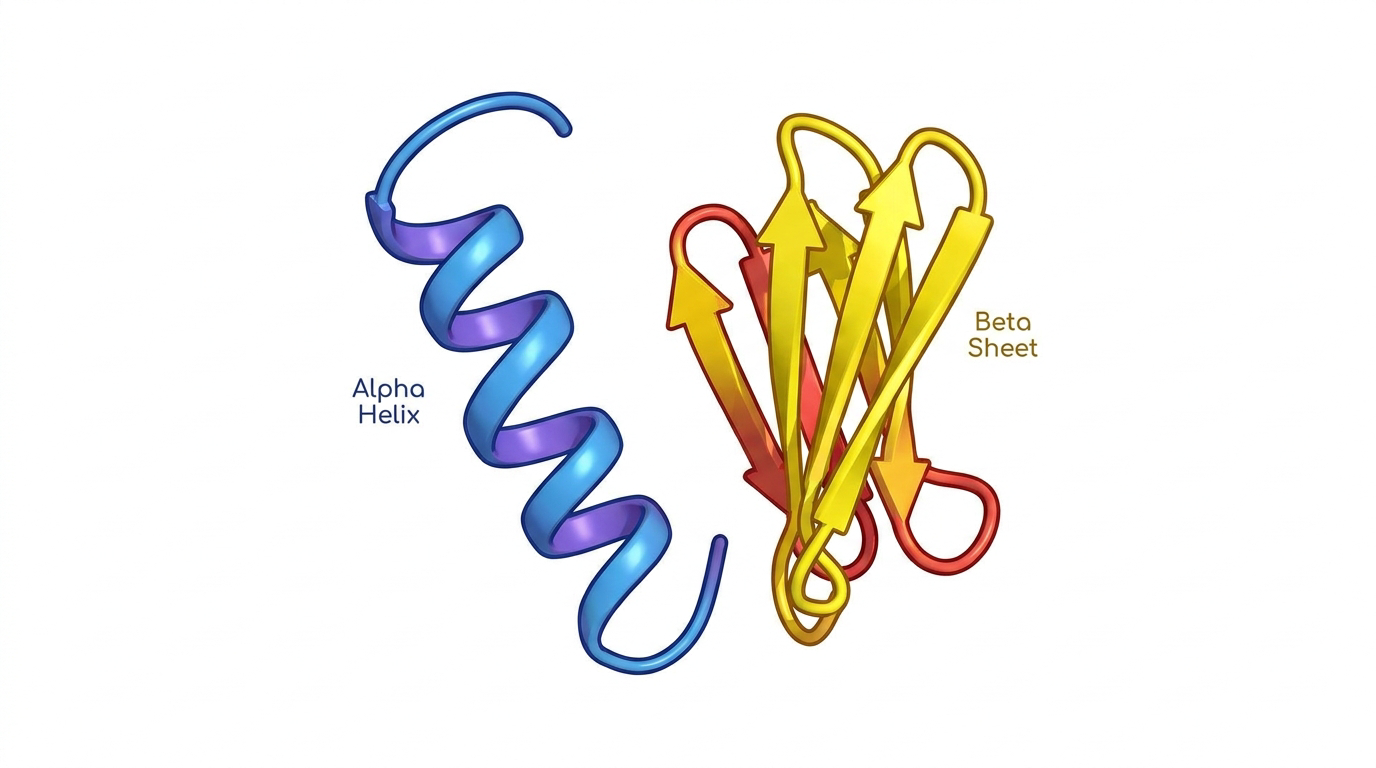
\includegraphics[width=0.9\linewidth]{assets/figures/protein_cartoon.png}
			{\footnotesize\color{softgray} PyMOL-style cartoon: helices + sheets}
		\end{center}
	\end{columns}
\end{frame}

\begin{frame}{LJ Fluid --- What Your Trajectory Looks Like}
	\begin{center}
		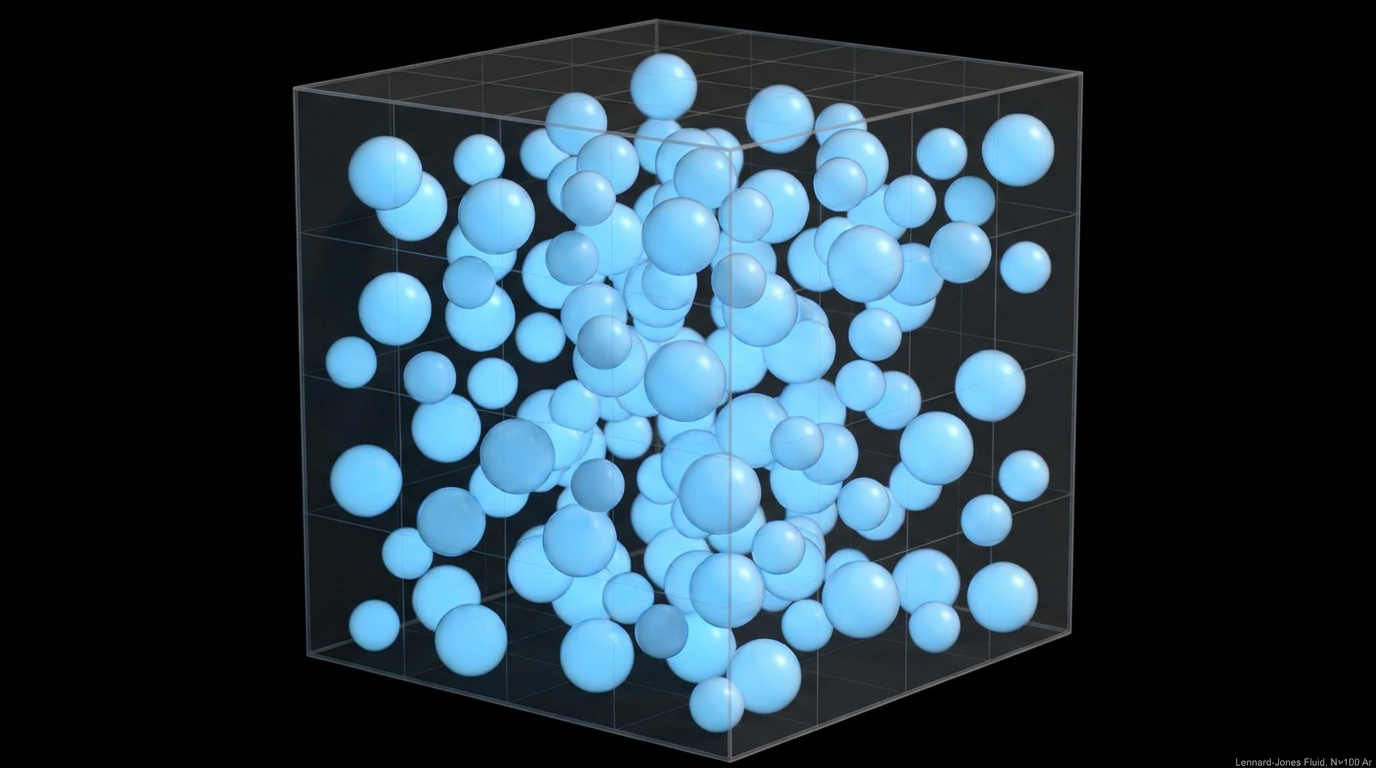
\includegraphics[width=0.7\linewidth]{assets/figures/lj_fluid_snapshot.png}
		{\footnotesize\color{softgray} Lennard-Jones fluid snapshot (OVITO view)}
	\end{center}
\end{frame}

\begin{frame}{Interpretation --- Analysis}
	\interpret{
		\textbf{trajectory} · movie · \textbf{RMSD} · drift · \textbf{RMSF} · flex · \textbf{$R_g$} · compact · \textbf{H-bond} · geometry · \textbf{$g(r)$} · shells · \textbf{clustering} · 5 states · \textbf{visualize} · trust
	}
\end{frame}
